\title{Rokkoチュートリアル}

\newtheorem{rei}{例}
\renewcommand{\therei}{}

\begin{document}

\lstset{language=c++,basicstyle=\ttfamily\tiny,showspaces=false,keepspaces=true,rulecolor=\color[cmyk]{0, 0.29,0.84,0}}

\begin{frame}
  \titlepage
  \noindent {\footnotesize PDFファイル: \url{http://sf.net/projects/rokko-tutorial/files/}} \\
  \noindent {\footnotesize LaTeXソース: \url{http://github.com/cmsi/rokko-tutorial/}}
\end{frame}

%% \section*{Outline}
%% \begin{frame}
%%   \tableofcontents
%% \end{frame}

\section{チュートリアルの概要}

\begin{frame}{Rokkoチュートリアル スタッフ}
  \begin{itemize}
  \item 講師
    \setlength{\itemsep}{1em}
    \begin{itemize}
      \setlength{\itemsep}{1em}
    \item 坂下達哉 (東大物性研) \ \href{mailto:t-sakashita@issp.u-tokyo.ac.jp}{t-sakashita@issp.u-tokyo.ac.jp}
    \item 藤堂眞治 (東大院理/物性研) \ \href{mailto:wistaria@phys.s.u-tokyo.ac.jp}{wistaria@phys.s.u-tokyo.ac.jp}
%    \item 五十嵐 亮 (東大物性研) \ \href{mailto:rigarash@issp.u-tokyo.ac.jp}{rigarash@issp.u-tokyo.ac.jp}
%    \item 本山裕一 (東大物性研) \ \href{mailto:y-motoyama@issp.u-tokyo.ac.jp}{y-motoyama@issp.u-tokyo.ac.jp}
    \end{itemize}
  \item 主催
    \begin{itemize}
    \item CMSI: 計算物質科学イニシアティブ \url{http://cms-initiative.jp/}
    \end{itemize}
  \end{itemize}
\end{frame}

\begin{frame}
  \frametitle{チュートリアルの流れ}
  \begin{itemize}
    %\setlength{\itemsep}{1em}
  \item 座学: 既存の固有値問題の解法・固有値ソルバ/線形計算ライブラリ
  \item 座学: Rokkoの概要と内部構造
  \item 実習: Rokkoのインストール
  \item 座学・実習: 密行列向け逐次ソルバの基本概念、サンプル実行
  \item 座学・実習: 密行列向けMPI並列ソルバの基本概念、サンプル実行
  \item 座学・実習: 疎行列向けMPI並列ソルバの基本概念、サンプル実行
  \item 実習: 量子スピン系の対角化のサンプル実行
  \item 実習: TITPACK2へのRokko組み込み実習
  \item 実習: アプリケーションからのRokkoの利用
%  \item (付録: ALPS/Baristaパッケージ)
 % \item (付録: MateriAppsとMateriApps LIVE!)
  \end{itemize}
\end{frame}

\begin{frame}
  \frametitle{ネットワーク設定(別紙参照)}
  \begin{itemize}
    \setlength{\itemsep}{1em}
  \item LAN接続 (無線 or 有線)
  \item 講習会資料ダウンロード
  \item 実習用ワークステーションのアカウント登録
  \item 実習用ワークステーションへのログイン確認
  \end{itemize}
\end{frame}

\section{固有値問題の解法・固有値ソルバ/線形計算ライブラリ}

\begin{frame}
  \frametitle{固有値問題の解法・固有値ソルバ/線形計算ライブラリ}
  \begin{itemize}
    \setlength{\itemsep}{1em}
  \item 行列の対角化
  \item 固有値問題の解法
  \item 既存の固有値ソルバ/線形計算ライブラリ
  \end{itemize}
\end{frame}

\begin{frame}
  \frametitle{行列の対角化}
  \begin{itemize}
    %\setlength{\itemsep}{1em}
  \item 行列の種類
    \begin{itemize}
    \item 実対称行列, 実非対称行列, エルミート行列, 非エルミート行列
    \end{itemize}
  \item 行列の表示
    \begin{itemize}
      \item 密行列, CRS(Compressed Row Storage)形式, MatFree形式\\
            (それぞれTITPACK2の「小規模」, 「中規模」, 「大規模」に対応)
    \end{itemize}
  \item 必要な固有値
    \begin{itemize}
      \item 全て, 絶対値の大きな(小さな)順にいくつか, ある範囲内
    \end{itemize}
  \item 固有ベクトル
    \begin{itemize}
      \item 要/不要
    \end{itemize}
  \end{itemize}
\end{frame}

\begin{frame}
  \frametitle{用語の定義}
  \begin{itemize}
    %\setlength{\itemsep}{1em}
  \item 固有値問題の解法(Eigenvalue algorithm)
    \begin{itemize}
      \item 固有値問題を解くためのアルゴリズム
    \end{itemize}
  \item 固有値ソルバ(Eigensolver, Eigenvalue problem solver)
    \begin{itemize}
      \item 固有値解法の実装
    \end{itemize}
  \item 固有値ソルバライブラリ(Eigensolver Library)
    \begin{itemize}
      \item 固有値ソルバのみを含むライブラリ
    \end{itemize}
  \item 線形計算ライブラリ(Linear Algebra Library)
    \begin{itemize}
      \item 固有値ソルバや他の線形計算ソルバの集合体
    \end{itemize}
  \item 厳密対角化パッケージ(Exact diagonalization package)
    \begin{itemize}
      \item 量子格子模型のハミルトニアンの固有値問題を扱うソフトウェア
    \end{itemize}
  \end{itemize}
\end{frame}

\begin{frame}
  \frametitle{固有値問題の解法(一部)}
  \begin{itemize}
    %\setlength{\itemsep}{1em}
  \item 三重対角行列に対する固有値問題の解法
    \begin{itemize}
      \item 二分法, QR法, MR3, 分割統治法+QR法
    \end{itemize}
  \item 密行列の直接対角化
    \begin{itemize}
      \item Jacobi法
    \end{itemize}
  \item 密行列の三重対角化
    \begin{itemize}
      \item Householder法
    \end{itemize}
  \item 疎行列の直接対角化
    \begin{itemize}
      \item べき乗法, 逆べき乗法, レイリー商反復法, Jacobi-Davidson法, LOBPCG, Krylov-Schur法
    \end{itemize}
  \item 疎行列の三重対角化
    \begin{itemize}
      \item Lanczos法, Arnoldi法, リスタート付きLanczos法(Restart Lanczos), Thick-restart Lanczos法
    \end{itemize}
  \item その他の方法
    \begin{itemize}
      \item Sakurai-Sugiura法
    \end{itemize}
  \end{itemize}
\end{frame}

\begin{frame}
  \frametitle{固有値問題の解法}
  \begin{center}
    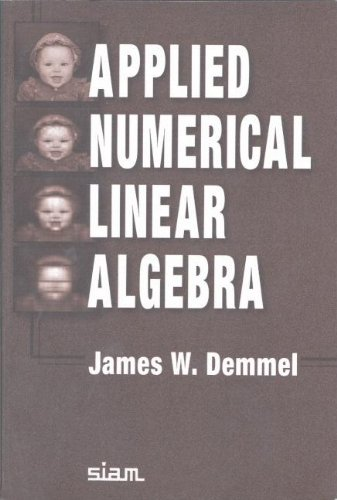
\includegraphics[height=0.45\textheight]{figure/AppliedNumericalLinearAlgebra.jpg} \ \
    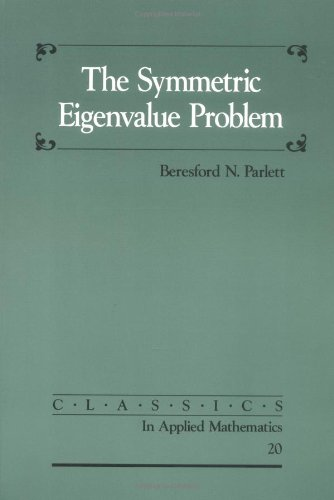
\includegraphics[height=0.45\textheight]{figure/TheSymmetricEigenvalueProblem.jpg} \ \
    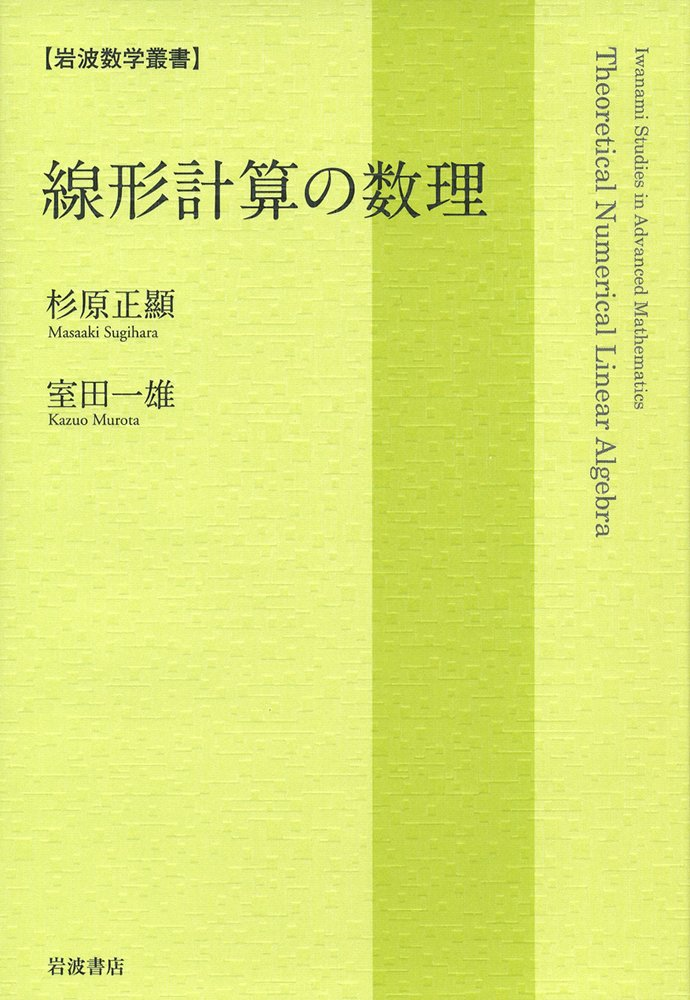
\includegraphics[height=0.45\textheight]{figure/SenkeikeisanNoSuri.jpg}  \ \
    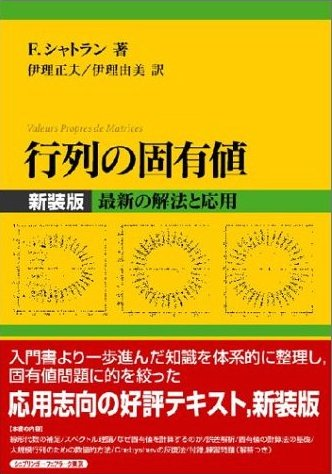
\includegraphics[height=0.45\textheight]{figure/GyoretsuNoKoyuchi.jpg}
  \end{center}
\end{frame}

\begin{frame}
  \frametitle{既存の固有値ソルバライブラリ(密行列向け)}
  \begin{itemize}
    %\setlength{\itemsep}{1em}
  \item EigenExa: 密行列ソルバ
    \begin{itemize}
      \item Householder (3重対角化, 5重対角化)+分割統治法+QR
    \end{itemize}
  \item ELPA
    \begin{itemize}
      \item Householder+分割統治法+QR
    \end{itemize}
  \end{itemize}
\end{frame}

\begin{frame}
  \frametitle{既存の固有値ソルバライブラリ(疎行列向け)}
  \begin{itemize}
  \item Anasazi: 反復法ソルバ中心
    \begin{itemize}
      \item Krylov-Schur, Jacobi-Davidson, XXX-Davidson, LOBPCG, Implicit Riemannian Trust Region Method
    \end{itemize}
  \item ARPACK
    \begin{itemize}
      \item Implicit Restarted Lanczos
    \end{itemize}
  \item BLOPEX
    \begin{itemize}
    \item Locally Optimal Block Preconditioned Conjugate Gradient Method (LOBPCG)
    \end{itemize}
  \item SLEPc: 反復法ソルバ中心, ビルド時に逐次かMPI並列かを選ぶ必要あり
    \begin{itemize}
      \item Krylov-Schur, Generalized Davidson, Jacobi-Davidson, Rayleigh Quotient Conjugate Gradient, Contour integral Sakurai-Sugiura, Power method, Subspace Itertation, Arnoldi (explicit restart), Lanczos (explicit restart) \\
    \end{itemize}
  \item IETL: ALPSに含まれる反復法ソルバ
    \begin{itemize}
      \item Lanczos, 他
    \end{itemize}
  \end{itemize}
\end{frame}

\begin{frame}
  \frametitle{既存の線形計算ライブラリ(密行列向け)}
  \begin{itemize}
    %\setlength{\itemsep}{1em}
  \item LAPACK, ScaLAPACKのベンダ実装
    \begin{itemize}
    \item Apple VecLib: LAPACK
    \item Fujitsu SSLII: LAPACK, ScaLAPACK(の一部), 他
    \item Intel MKL: LAPACK, ScaLAPACK
    \end{itemize}
  \item Netlib LAPACK: LAPACKのリファレンス実装
    \begin{itemize}
      \item Householder+QR, Householder+分割統治法+QR, Householder+二分法, Householder+MR3
    \end{itemize}
  \item Netlib ScaLAPACK: ScaLAPACKのリファレンス実装
    \begin{itemize}
      \item Householder+QR, Householder+分割統治法+QR, Householder+二分法, Householder+MR3
    \end{itemize}
  \item Eigen3(逐次版、行列・行列積のみスレッド並列化)
    \begin{itemize}
      \item Householder+QR
    \end{itemize}
  \item Elemental:含まれる固有値ソルバMRRRは、プロセス数が平方数の場合のみ確実に動く
    \begin{itemize}
      \item Householder+MR3
    \end{itemize}
  \end{itemize}
\end{frame}

\begin{frame}
  \frametitle{既存の線形計算ライブラリ(疎行列向け)}
  \begin{itemize}
    %\setlength{\itemsep}{1em}
  \item Trilinos:固有値ソルバライブラリAnasaziを含む
  \item Xabclib (ppOpen AT)
  \end{itemize}
\end{frame}

\begin{frame}
  \frametitle{おすすめ順}
  \begin{itemize}
    %\setlength{\itemsep}{1em}
  \item 密行列・逐次
    \begin{itemize}
      \item LAPACK (のベンダ実装) $>$ Eigen3
    \end{itemize}
  \item 密行列・MPI並列
    \begin{itemize}
      \item EigenExa $>$ ELPA $>$ ScaLAPACK (のベンダ実装) $>$ Elemental
    \end{itemize}
  \item 疎行列(逐次、MPI並列)
    \begin{itemize}
      \item Anasazi $>$ SLEPc
    \end{itemize}
  \end{itemize}
\end{frame}

\begin{frame}{EigenExaによる超巨大密行列の対角化}
  \begin{center}
    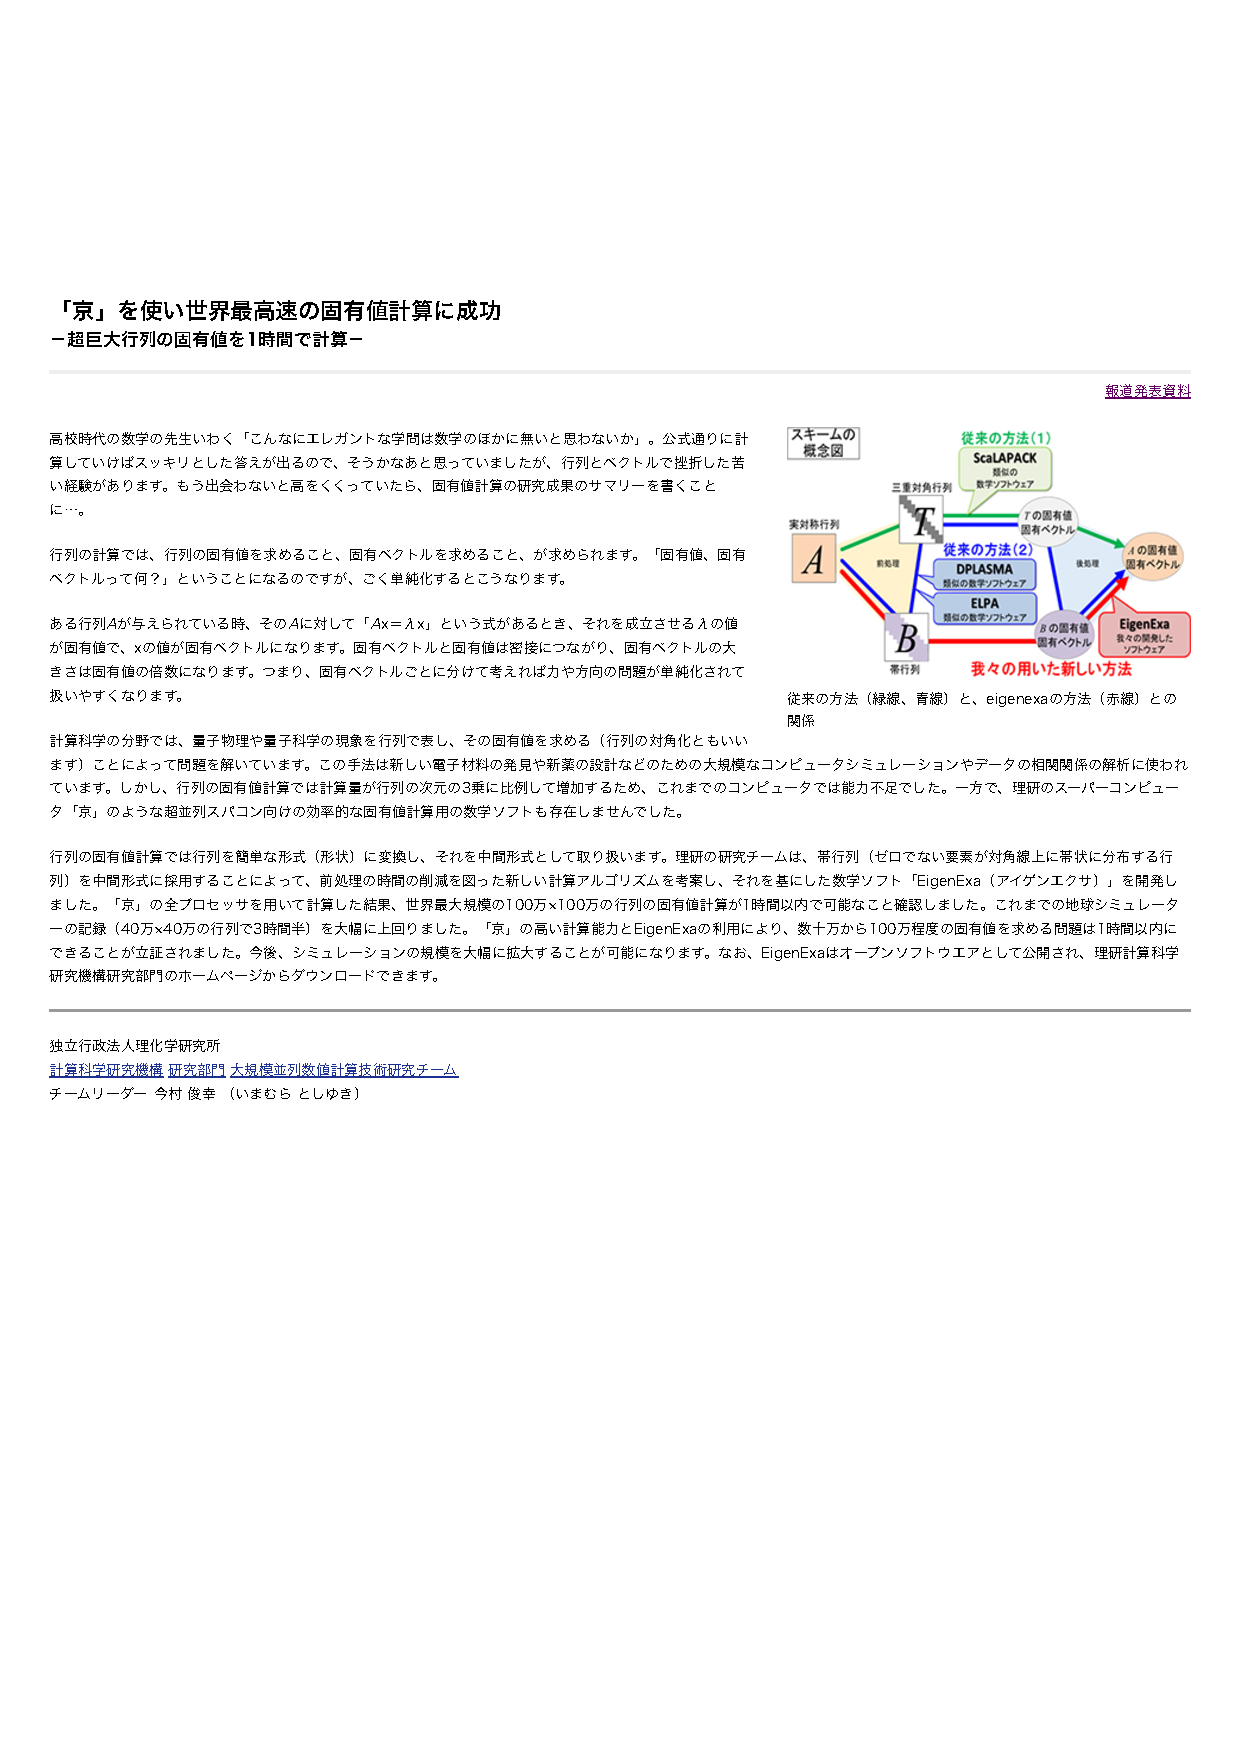
\includegraphics[height=0.8\textheight]{figure/eigenexa.pdf}
  \end{center}
\end{frame}

\begin{frame}
  \frametitle{最新の固有値ソルバ}
  \begin{itemize}
    \setlength{\itemsep}{1em}
  \item ハイブリッド並列(MPI+OpenMP)対応のソルバも増えてきた
  \item 超並列環境に対応した並列ソルバをユーザ自身が実装・最適化するの
    はもはや不可能
  \item 最新の並列固有値ソルバを積極的に活用すべき
  \end{itemize}
\end{frame}

\begin{frame}
  \frametitle{厳密対角化パッケージの状況}
  \begin{itemize}
    \setlength{\itemsep}{1em}
  \item 代表的なパッケージ
    \begin{itemize}
    \item ALPS(fulldiag/sparsediag): LAPACK, IETLを利用
    \item KOBEPACK: 独自の固有値ソルバを実装
    \item SPINPACK: LAPACKを利用
    \item TITPACK2: 独自の固有値ソルバを実装
    \end{itemize}
  \item 逐次 or スレッド並列のみ, MPI並列なし
  \item 最新の超並列スパコン環境を活かしきれていない
  \end{itemize}
\end{frame}

\begin{frame}
  \frametitle{固有値解法とソルバ}
  \begin{itemize}
    \setlength{\itemsep}{1em}
    \item GitHub Wikiに, 固有値問題の解法, 固有値ソルバ, 固有値ソルバ/線形計算ライブラリ, 厳密対角化パッケージに関するリファレンス・マニュアルを作成中
      \begin{itemize}
        \item 固有値解法とソルバ: \url{https://github.com/t-sakashita/rokko/wiki/EigenvalueAlgorithms}
      \end{itemize}
    \item ボランティア募集中!
  \end{itemize}
\end{frame}
        
\section{Rokkoの概要と内部構造}

\begin{frame}
  \frametitle{Rokkoの概要と内部構造}
  \begin{itemize}
    \setlength{\itemsep}{1em}
  \item 既存のライブラリの問題点
  \item Rokkoの概要
  \item 並列ソルバの基本概念
  \item Rokkoの内部構造
  \end{itemize}
\end{frame}

\begin{frame}
  \frametitle{既存のライブラリの問題点}
  \begin{itemize}
    \setlength{\itemsep}{1em}
  \item ソルバ毎に異なるデザイン
  \item インストール方法もライブラリ毎に異なる
  \item ドキュメントが不十分な場合も多い
  \item コンピュータのアーキテクチャ毎に異なるコンパイル・リンクオプションが必要
  \item C++/C/Fortran相互リンクの問題
  \item ライブラリ間の依存関係が複雑
  \item 実際に試す前に大まかな性能比較が欲しい
  \end{itemize}
\end{frame}

\begin{frame}
  \frametitle{ライブラリ間の依存関係(密行列向け)}
  \begin{center}
    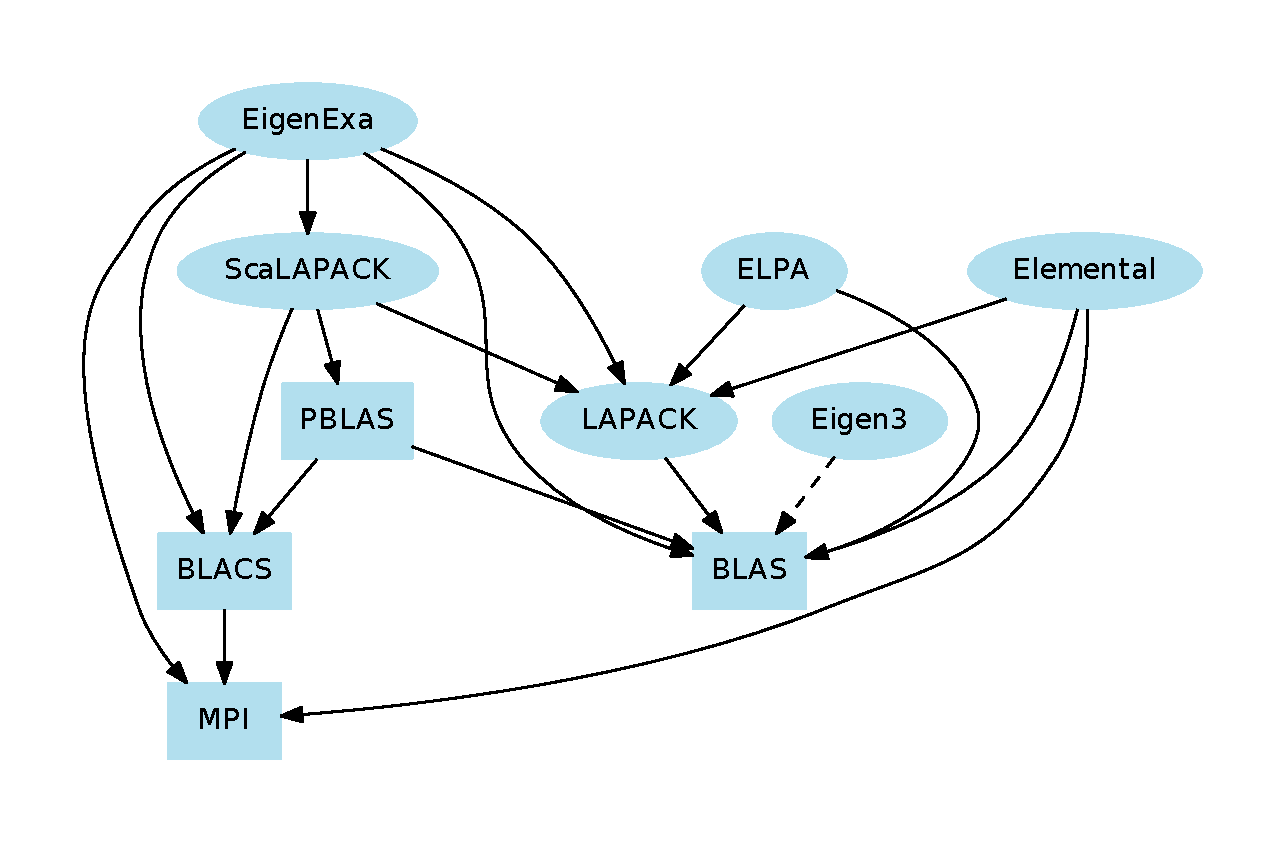
\includegraphics[height=0.8\textheight]{figure/eigensolver_dependency.pdf}
  \end{center}
\end{frame}

\begin{frame}
  \frametitle{Rokkoの開発者}
  \begin{itemize}
    \setlength{\itemsep}{1em}
  \item 坂下達哉 (東大物性研) \ \href{mailto:t-sakashita@issp.u-tokyo.ac.jp}{t-sakashita@issp.u-tokyo.ac.jp}
  \item 本山裕一 (東大物性研) \ \href{mailto:y-motoyama@issp.u-tokyo.ac.jp}{y-motoyama@issp.u-tokyo.ac.jp}
  \item 五十嵐 亮 (東大物性研) \ \href{mailto:rigarash@issp.u-tokyo.ac.jp}{rigarash@issp.u-tokyo.ac.jp}
  \item 大久保 毅 (東大物性研) \ \href{mailto:t-okubo@issp.u-tokyo.ac.jp}{t-okubo@issp.u-tokyo.ac.jp}
  \item 藤堂眞治 (東大院理/物性研) \ \href{mailto:wistaria@phys.s.u-tokyo.ac.jp}{wistaria@phys.s.u-tokyo.ac.jp}
  \end{itemize}
\end{frame}

\begin{frame}
  \frametitle{Rokkoの概要}
  \begin{itemize}
    %\setlength{\itemsep}{1em}
  \item 使用言語
    \begin{itemize}
      %\setlength{\itemsep}{1em}
    \item コア部分: C++
    \item 言語バインディング: C, Fortran90
    \item ベンチマークスクリプト: Python
    \end{itemize}
  \item ライセンス
    \begin{itemize}
      %\setlength{\itemsep}{1em}
    \item Boostライセンス (ほぼ自由に使える)
    \end{itemize}
  \item ソースコード
    \begin{itemize}
      %\setlength{\itemsep}{1em}
    \item GitHubで公開\\
          \url{https://github.com/t-sakashita/rokko/}
    \end{itemize}
  \end{itemize}
\end{frame}

\begin{frame}
  \frametitle{VCS (Version Control System)によるソース管理}
  \begin{itemize}
  \item 開発者が複数になると, ディレクトリ名やログファイルによるバージョン管理はすぐに破綻する
  \item ソースコードをサーバー上で一括管理
    \begin{itemize}
    \item ネットワーク経由でソースを check out/check in
    \end{itemize}
  \item 全ての修正履歴を保存
  \item 複数人が同時に更新した場合に衝突を回避するしくみ
  \item ブランチ・マージ・タグ付けなどが可能
  \item 開発者が一人, 公開の予定がない場合でも積極的に使うべき
  \item 参考資料: バージョン管理web講習会 {\tiny \url{http://www.cms-initiative.jp/ja/research-support/develop-support/how-to-publish/develop-apps/manage-version}}
  \end{itemize}
\end{frame}

\begin{frame}
  \frametitle{Rokkoの設計方針}
  \begin{itemize}
    \setlength{\itemsep}{1em}
  \item 共通のベクトルや行列クラス
  \item ソルバの違いはラッパーで吸収
    \begin{itemize}
      %\setlength{\itemsep}{1em}
    \item 個々のソルバに仕様変更があってもRokkoが吸収
    \end{itemize}
  \item 再コンパイルなしに, 実行時にソルバを選択可能
  \item 仮想関数とテンプレートを組み合わせることで, オーバーヘッドの少ないラッパーを実装
  \item C++, C, Fortran90から使用可能に
  \end{itemize}
\end{frame}

\begin{frame}
  \frametitle{Rokkoの全体像}
  \begin{itemize}
    %\setlength{\itemsep}{1em}
  \item 固有値ソルバ/線形演算ライブラリのインストールスクリプト
  \item 共通基本クラス(分散行列, プロセスグリッド他)
  \item 固有値ソルバラッパー(C++)
  \item 固有値ソルバ・ファクトリ(C++)
  \item C/Fortranラッパー
  \item テスト・サンプルプログラム
  \item ベンチマークスクリプト
  \end{itemize}
\end{frame}

\begin{frame}
  \frametitle{Rokko Software Stack}
  \begin{center}
    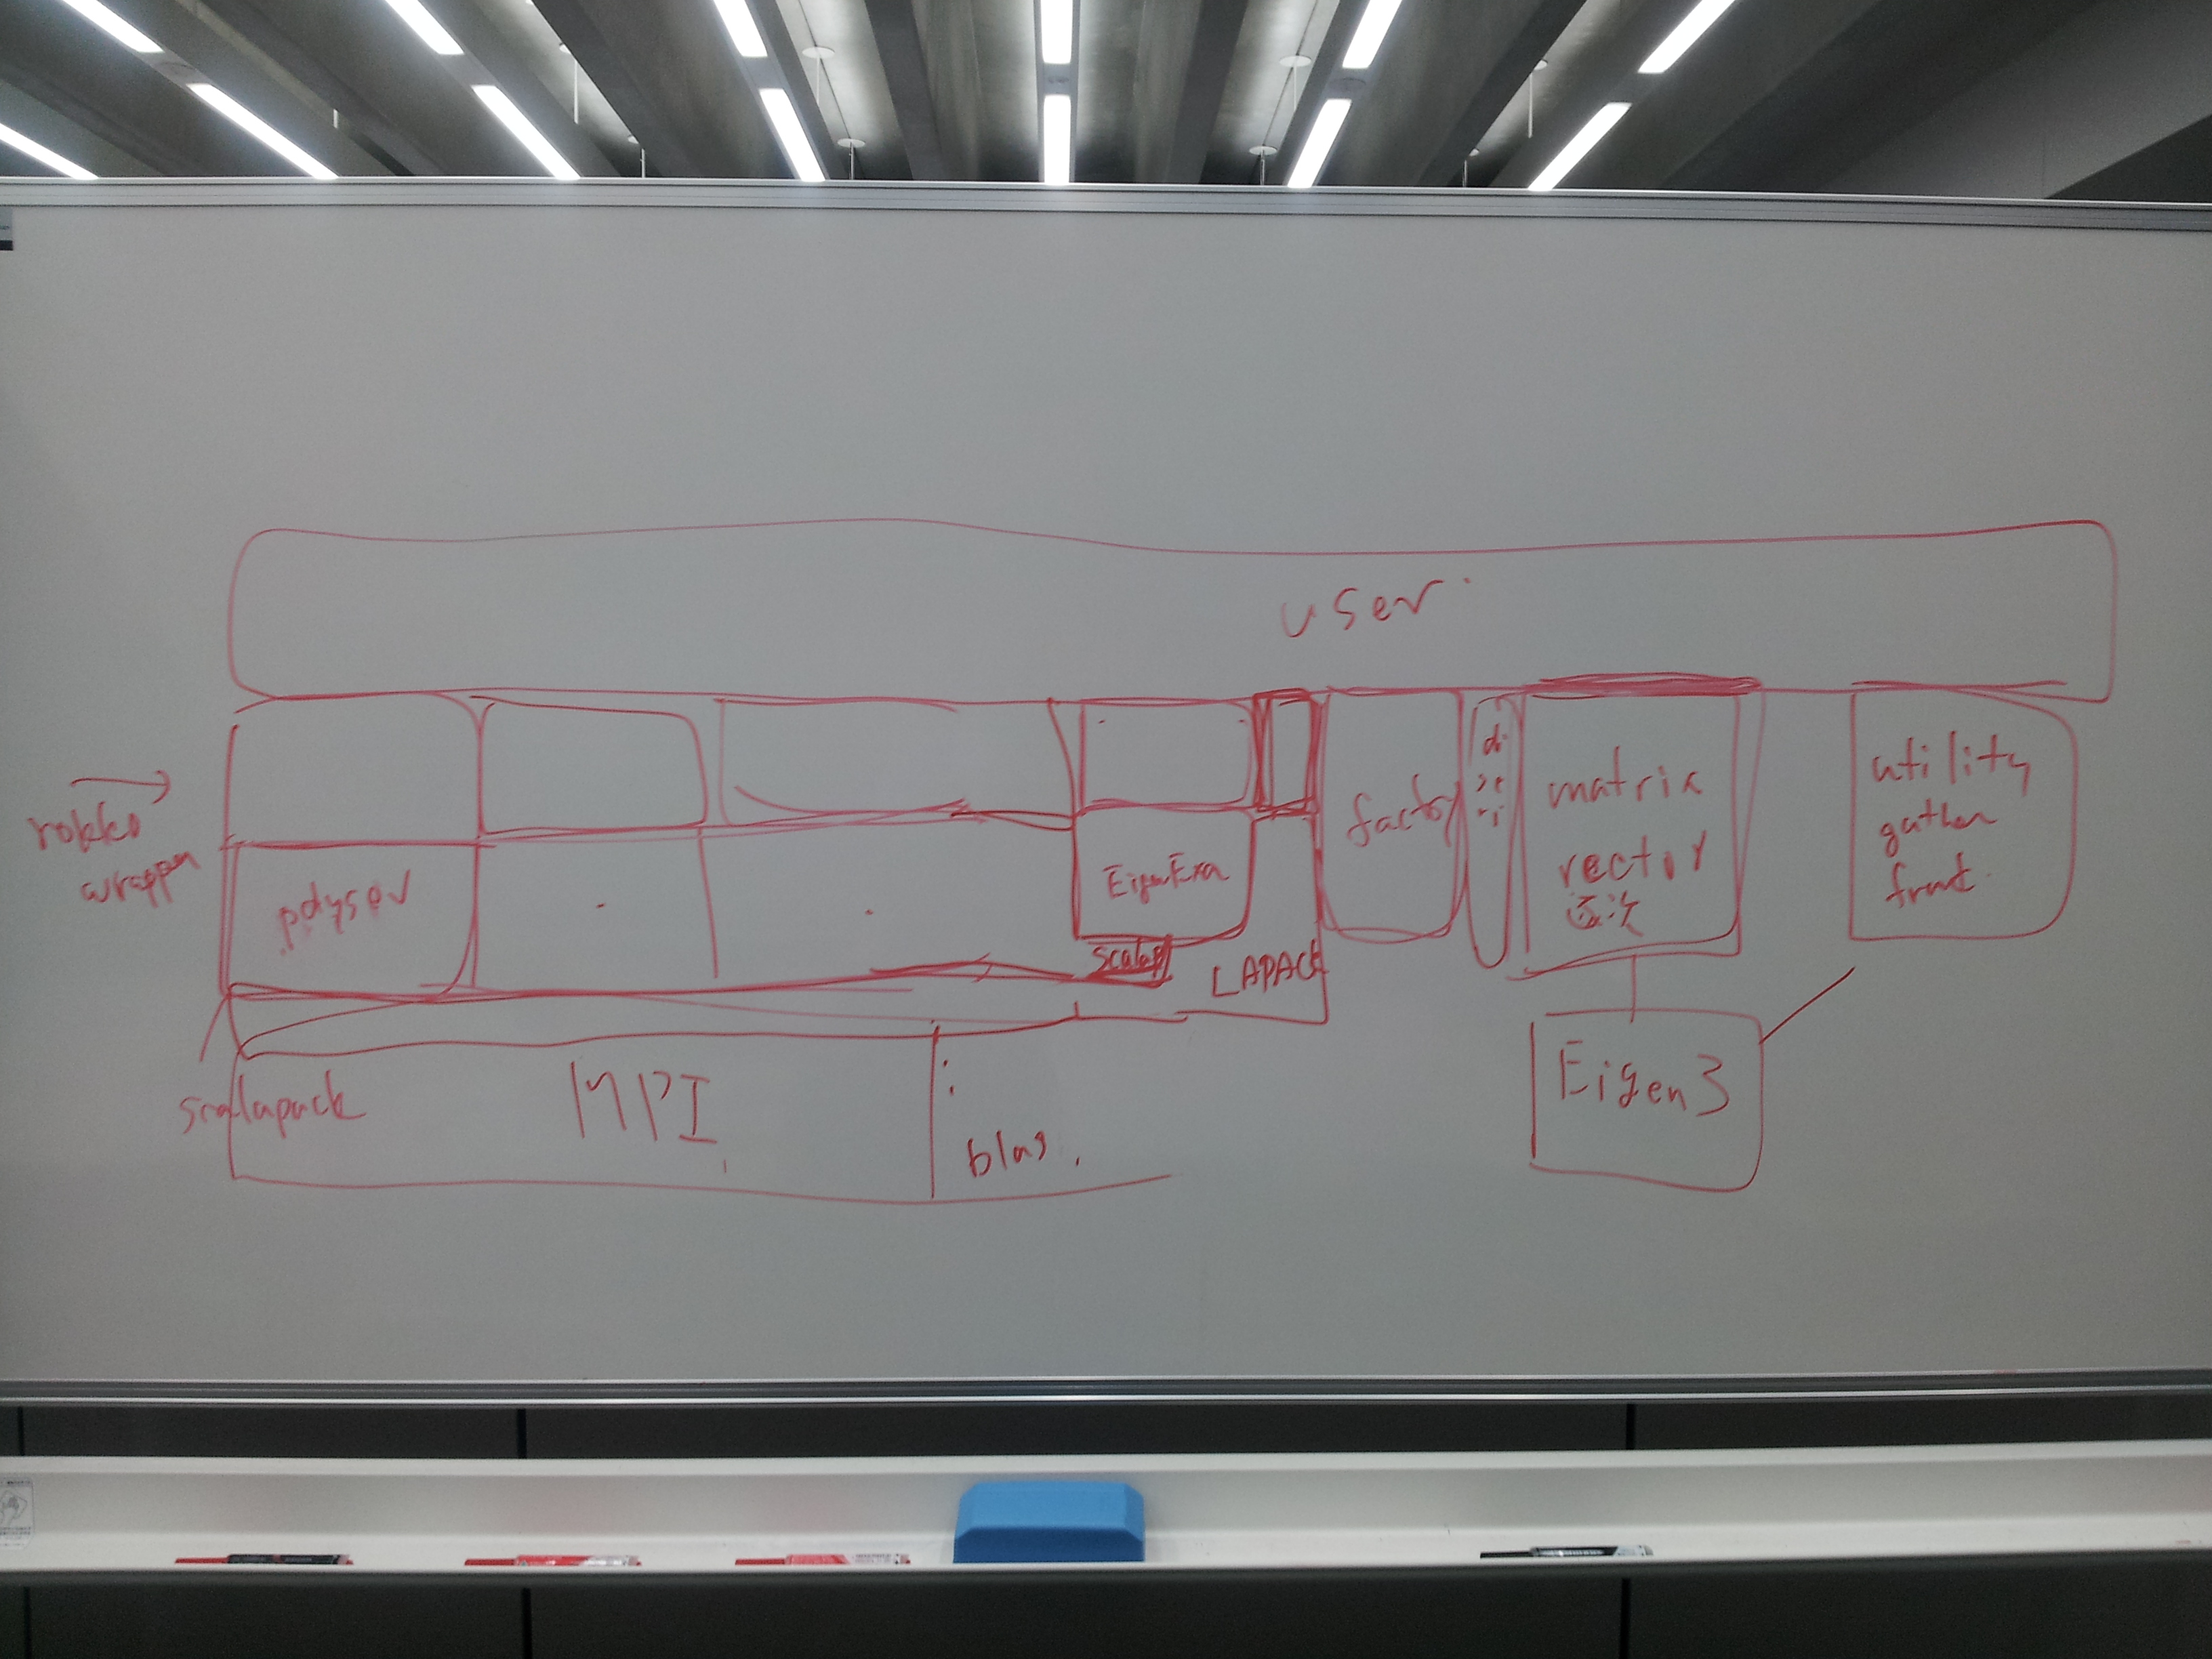
\includegraphics[height=0.8\textheight]{figure/rokko-software-stack.jpg}
  \end{center}
\end{frame}

\section{Rokkoのインストール}

\begin{frame}
  \frametitle{インストール作業に必須のツールとライブラリ}
  \begin{itemize}
    \setlength{\itemsep}{1em}
  \item CMake: \url{http://www.cmake.org}
  \item Boost C++ Libraries: \url{http://www.boost.org}
  \item インストールスクリプト: \url{https://github.com/wistaria/installer}
  \item 主要なスパコンへのインストール状況 \\
    \url{https://github.com/wistaria/installer/wiki}
  \end{itemize}
\end{frame}

\begin{frame}
  \frametitle{ビルドシステム: CMake}
  \begin{itemize}
    \setlength{\itemsep}{1em}
  \item Makefileを生成するためのユーティリティー (configureスクリプトに対応)
    \begin{itemize}
    \item Windows の Visual C++ 用ソリューションファイル, Mac OS X の Xcode 用プロジェクトファイルの生成も可能
    \end{itemize}
  \item 設定は CMakeLists.txt に記述する
  \item テスト(CTest)やバイナリ配布(CPack)の機能もある
  \item ファイルの依存関係の自動検出
  \item ソースディレクトリとビルドディレクトリの分離(バージョン管理がしやすくなる)
  \end{itemize}
\end{frame}

\begin{frame}
  \frametitle{サードパーティーの固有値ソルバ/線形計算ライブラリのインストール}
  \begin{itemize}
    \setlength{\itemsep}{1em}
  \item Eigen3 (ベクトル, 行列クラスを内部で利用), LAPACKE (LAPACKのCインターフェース)は, Rokkoに同梱されている
  \item インストールスクリプト: \href{https://github.com/t-sakashita/rokko/tree/master/3rd-party/install}{3rd-party/install}
    \begin{itemize}
      \item ライブラリ: Anasazi, EigenExa, Elemental, ELPA, PETSc, ScaLAPACK, SLEPc
      \item 対応アーキテクチャ: 京/FX10, x86スパコン・クラスタ(Intelコンパイラ/GCC), Mac OS X (GCC), 他
    \end{itemize}
  \item 主要なスパコンにインストール済み: \url{https://github.com/t-sakashita/rokko/wiki/PreInstall}
  \end{itemize}
\end{frame}

\begin{frame}[c,fragile]
  \frametitle{Rokkoのインストール}
  \begin{itemize}
    %\setlength{\itemsep}{1em}
  \item 下準備 (phi.aics.riken.jpの場合)
\begin{lstlisting}[style=shstyle]
source /opt/nano/alps/alpsvars.sh
\end{lstlisting}
  \item ソースコードのダウンロード・展開
\begin{lstlisting}[style=shstyle]
cd $HOME
wget --no-check-certificate https://github.com/t-sakashita/rokko/archive/0.2.tar.gz -O rokko-0.2.tar.gz
tar zxvf rokko-0.2.tar.gz
\end{lstlisting}
  \item CMake(のコマンドが書かれたスクリプトを実行)
\begin{lstlisting}[style=shstyle]
mkdir rokko-build
cd rokko-build
cp /home/hands-on/rokko_20140918/cmake-rokko.sh  .
bash ./cmake-rokko.sh
\end{lstlisting}
  \item Make, テスト
\begin{lstlisting}
make -j 10
make test
make install
\end{lstlisting}
  \end{itemize}
\end{frame}

\begin{frame}[c,fragile]
  \frametitle{インストールの成否の確認}
Rokkoで使用できる固有値ルーチン一覧の表示
\begin{lstlisting}[style=shstyle]
cd rokko/tool
./rokko_solvers
\end{lstlisting}

出力結果
\begin{lstlisting}[style=shstyle]
[serial dense solvers]
  eigen3
  lapack
[parallel dense solvers]
  eigen_exa_s
  eigen_exa_sx
  scalapack
  scalapack_pdsyevd
[parallel sparse solvers]
  anasazi
  slepc
\end{lstlisting}

\end{frame}

\begin{frame}[c,fragile]
  \frametitle{Rokkoのディレクトリ構造}

\dirtree{%
 .1 \href{https://github.com/t-sakashita/rokko/tree/develop}{rokko}.
 .2
 \href{https://github.com/t-sakashita/rokko/tree/develop/rokko}{rokko}
 $\cdots$ Rokko本体(ヘッダファイル・ソースファイル).
 .2
 \href{https://github.com/t-sakashita/rokko/tree/develop/sample}{sample}
 $\cdots$ C++によるサンプルプログラム.
 .3
 \href{https://github.com/t-sakashita/rokko/tree/develop/sample/dense}{dense}
 $\cdots$ 密行列用(逐次版、MPI版).
 .3 \href{https://github.com/t-sakashita/rokko/tree/develop/sample/sparse}{sparse} $\cdots$ 疎行列用(MPI版).
 .2 \href{https://github.com/t-sakashita/rokko/tree/develop/sample_c}{sample\_c} $\cdots$ Cによるサンプルプログラム.
 .3 \href{https://github.com/t-sakashita/rokko/tree/develop/sample_c/dense}{dense} $\cdots$ 密行列用(逐次版、MPI版).
 .3
 \href{https://github.com/t-sakashita/rokko/tree/develop/sample_c/sparse}{sparse}
 $\cdots$ 疎行列用(MPI版).
 .2 \href{https://github.com/t-sakashita/rokko/tree/develop/sample_fortran}{sample\_fortran}
 $\cdots$ Fortranによるサンプルプログラム.
 .3 \href{https://github.com/t-sakashita/rokko/tree/develop/sample_fortran/dense}{dense} $\cdots$ 密行列用(逐次版、MPI版).
 .3 \href{https://github.com/t-sakashita/rokko/tree/develop/sample_fortran/sparse}{sparse} $\cdots$ 疎行列用(MPI版).
% .2
% \href{https://github.com/t-sakashita/rokko/tree/develop/test}{test}
% $\cdots$ ctest用(インストール成否の確認).
% .2 3rd-party $\cdots$ 固有値ソルバ.
 .2 \href{https://github.com/t-sakashita/rokko/tree/develop/tutorial}{tutorial} $\cdots$ チュートリアル.
 .3
 \href{https://github.com/t-sakashita/rokko/tree/develop/tutorial/titpack}{titpack}
 $\cdots$ 厳密対角化パッケージの書き換え.
}

\end{frame}

\section{密行列向け逐次ソルバ}

\subsection{Rokkoインターフェースの仕様}

\begin{frame}[c,fragile]
  \frametitle{rokko::localized\_matrix クラステンプレート}
  \begin{itemize}
  \item \href{https://github.com/t-sakashita/rokko/blob/master/rokko/localized_matrix.hpp}{rokko/localized\_matrix.hpp}
\begin{lstlisting}
namespace rokko {
template<typename MATRIX_MAJOR = rokko::matrix_row_major>
class localized_matrix {
public:
  typedef MATRIX_MAJOR major_type;
  localized_matrix();
  localized_matrix(int rows, int cols);
  template <typename T>
  localized_matrix(T const& other);
  template <typename T>
  matrix_type& operator=(T const& other);
  double operator[](int i, int j) const;
  double& operator[](int i, int j);
  int get_m_global() const;
  int get_n_global() const;
  int get_m_local() const;
  int get_n_local() const;
  bool is_gindex_myrow(const int& global_i) const;
};
}
\end{lstlisting}
  \end{itemize}
\end{frame}

\begin{frame}[c,fragile]
  \frametitle{rokko::localized\_vector と rokko::localized\_matrix の利用例}
  \begin{itemize}
  \item \href{https://github.com/t-sakashita/rokko/blob/master/test/localized_matrix.cpp}{test/localized\_matrix.cpp}
\begin{lstlisting}
int dim = 3;
rokko::localized_matrix<> M(dim,dim);
M << 1,2,3,4,5,6,7,8,9;
double a = 5.0;
rokko::localized_vector u(dim);
u << 1,2,3;
rokko::localized_vector v(dim);
v << 4,5,6;
rokko::localized_vector w = a*u+M*v;
\end{lstlisting}
  \end{itemize}
\end{frame}

\begin{frame}[c,fragile]
  \frametitle{rokko::serial\_dense\_solverクラス}
  \begin{itemize}
    %\setlength{\itemsep}{1em}
  \item 初期化
\begin{lstlisting}
rokko::serial_dense_solver solver(name);
solver.initialize(argc, argv);
solver.finalize();
\end{lstlisting}
  \item 対角化 (行列は破壊される)
\begin{lstlisting}
rokko::localized_matrix<matrix_col_major> mat(dim, dim, solver);
...
rokko::localized_vector evals(dim);
rokko::localized_matrix<matrix_col_major> evecs(dim, dim, solver);
solver.diagonalize(mat, evals, evecs);
\end{lstlisting}
%  \item 登録されているソルバの一覧
%\begin{lstlisting}
%std::vector<std::string> names = rokko::serial_dense_solver::solvers();
%\end{lstlisting}
  \end{itemize}
\end{frame}

\subsection{サンプルの実行}

\begin{frame}[c,fragile]
  \frametitle{対角化のサンプル}
  \begin{itemize}
    %\setlength{\itemsep}{1em}
%  \item 逐次密行列ソルバーの一覧 \href{https://github.com/t-sakashita/rokko/blob/master/test/serial_dense_solvers.cpp}{test/serial\_dense\_solvers.cpp}
%\begin{lstlisting}[style=shstyle]
%./test/serial_dense_solvers
%\end{lstlisting}
  \item LAPACK dsyev を直接使う \href{https://github.com/t-sakashita/rokko/blob/master/sample/dense/dsyev.c}{sample/dense/dsyev.cpp}
\begin{lstlisting}[style=shstyle]
./sample/dense/dsyev
\end{lstlisting}
  \item 逐次密行列ソルバを使う \href{https://github.com/t-sakashita/rokko/blob/master/sample/dense/frank_dense.cpp}{sample/dense/frank.cpp}
\begin{lstlisting}[style=shstyle]
./sample/dense/frank lapack 5
\end{lstlisting}
  \end{itemize}
\end{frame}

\section{密行列向けMPI並列ソルバ}

\subsection{基本概念}

\begin{frame}
  \frametitle{2次元プロセスグリッド}
  \begin{itemize}
    %\setlength{\itemsep}{1em}
  \item MPIプロセスの2次元割付けを指定
  \item Row-majorとcolumn-majorの二種類
  \item 4プロセスの例 (左:row-major, 右:column-major)
  \begin{center}
    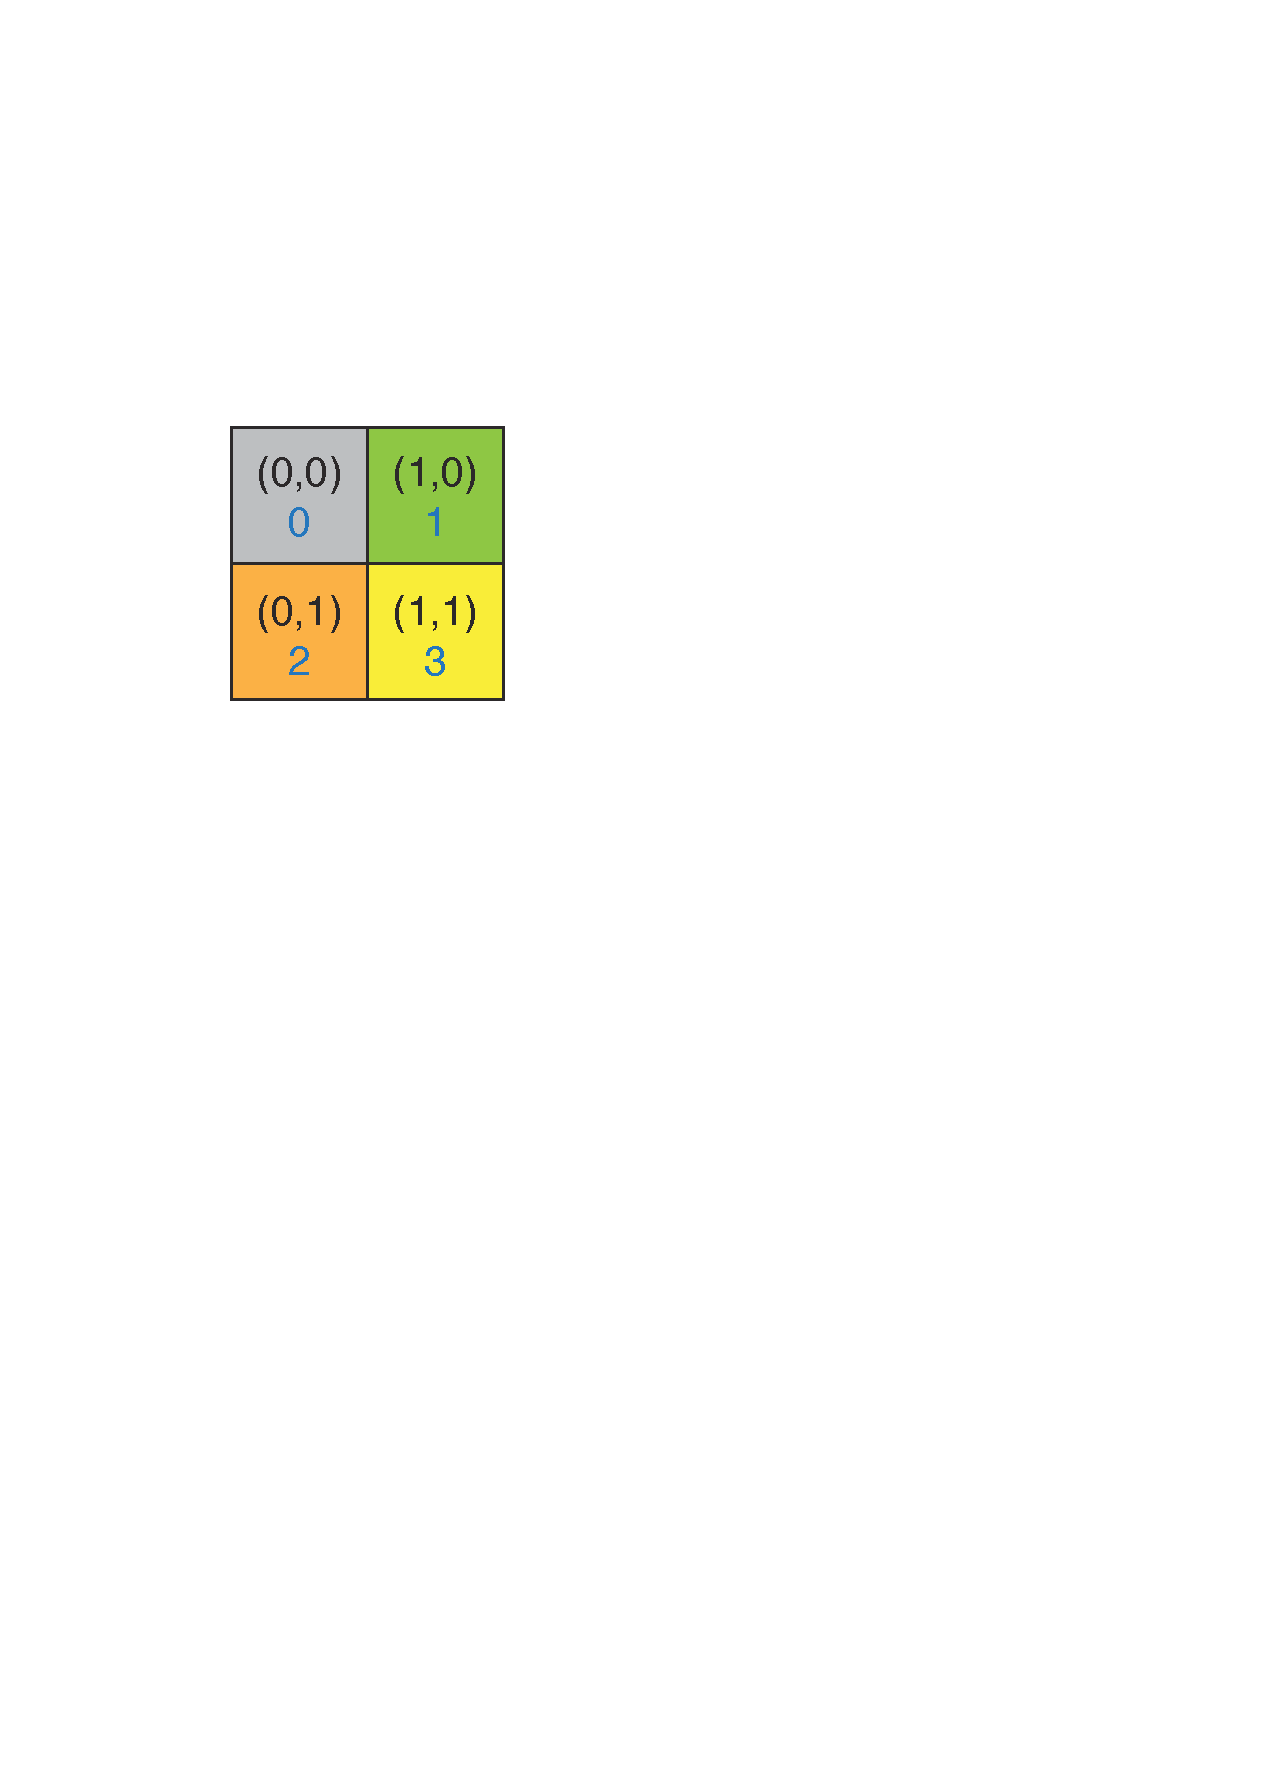
\includegraphics[height=0.25\textheight]{figure/grid-row-major.pdf} \ \ \ \
    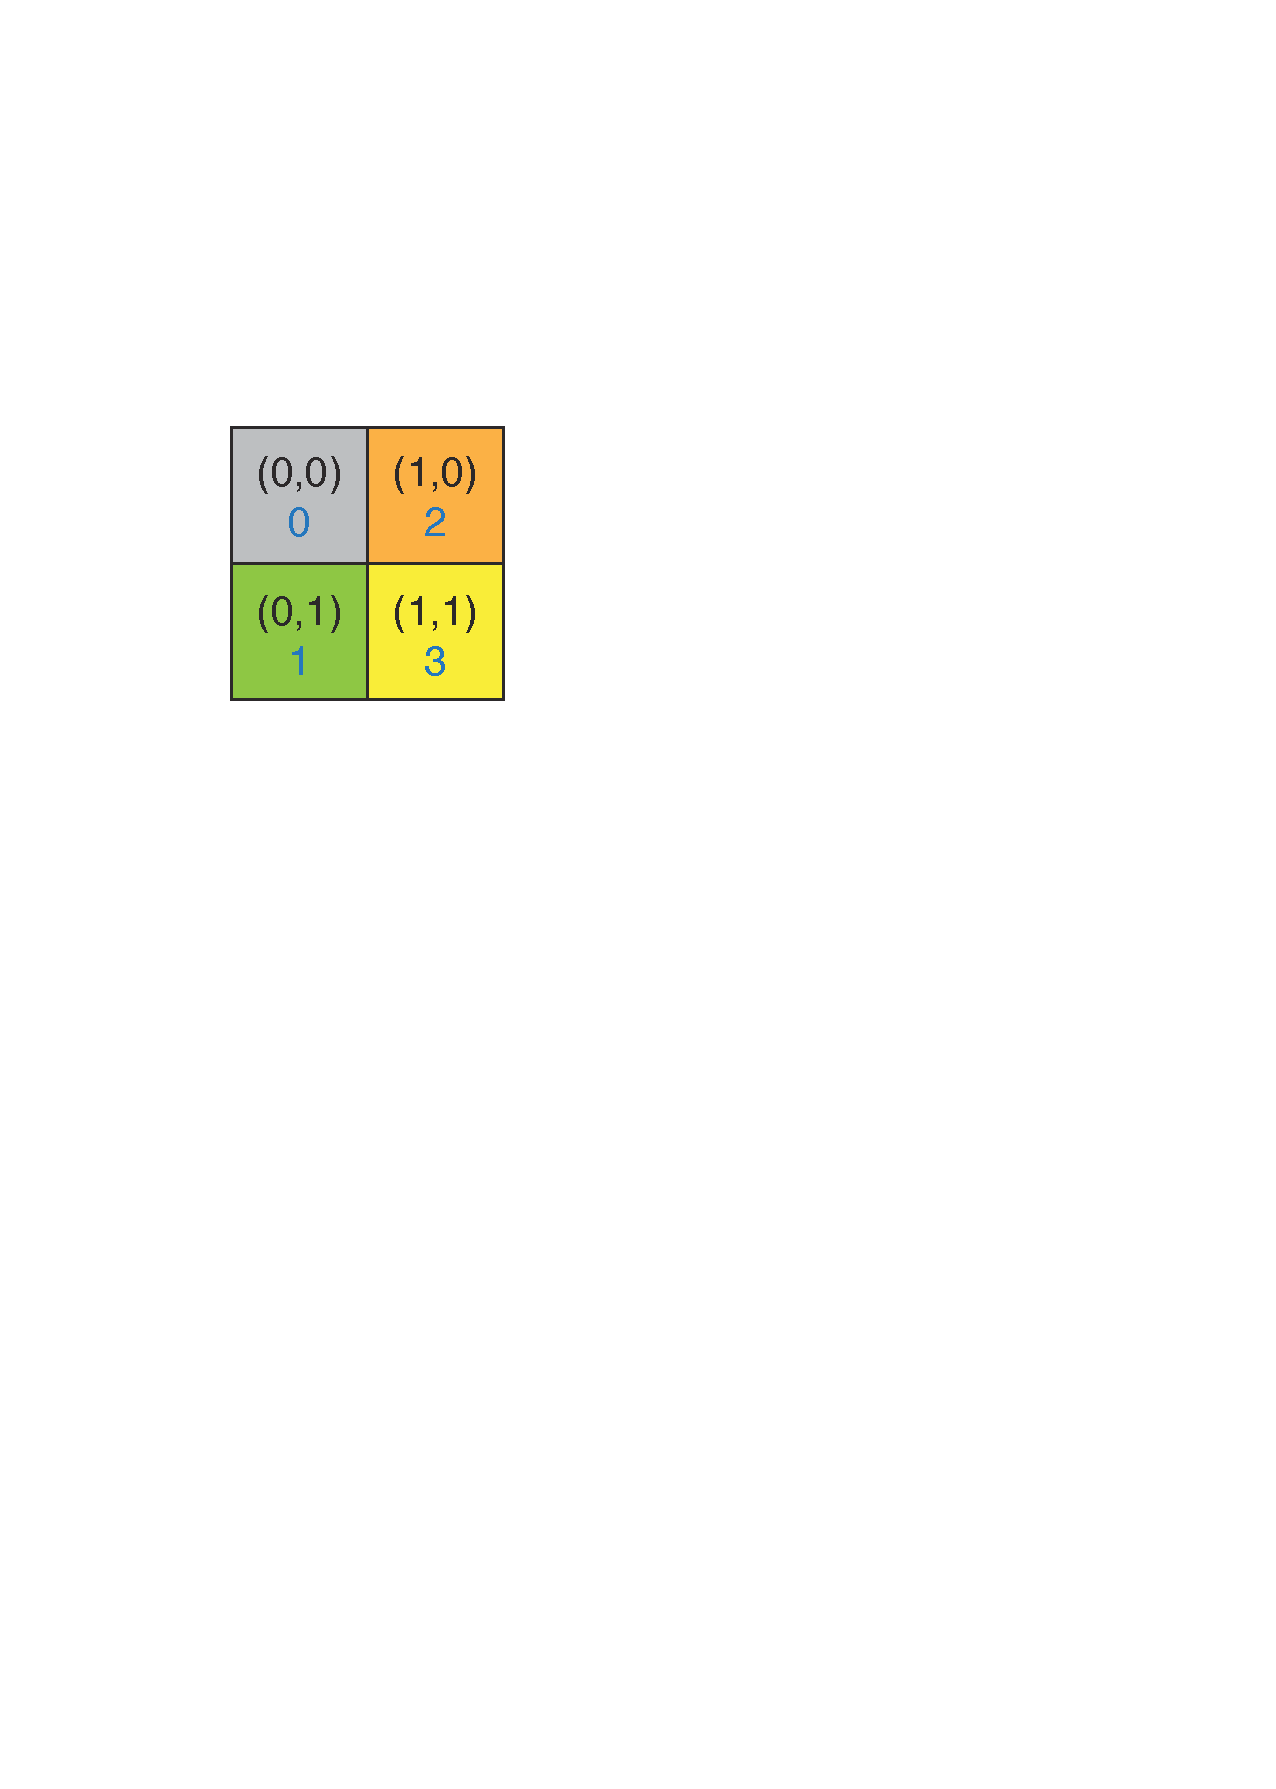
\includegraphics[height=0.25\textheight]{figure/grid-column-major.pdf}
  \end{center}
  \item ほとんどの並列固有値ソルバは両方の種類をサポート \\
    (Elementalはcolumn-majorのみサポート)
  \end{itemize}
\end{frame}

\begin{frame}
  \frametitle{2次元ブロック・サイクリック行列(distributed\_matrix)}
  \begin{itemize}
    %\setlength{\itemsep}{1em}
  \item ほとんどの並列固有値ソルバにおいて, 密行列は「2次元ブロック・サイクリック形式」でデータ分割される
  \item 4プロセスでの例 (左 ローカルビュー, 右 グローバルビュー)
  \begin{center}
    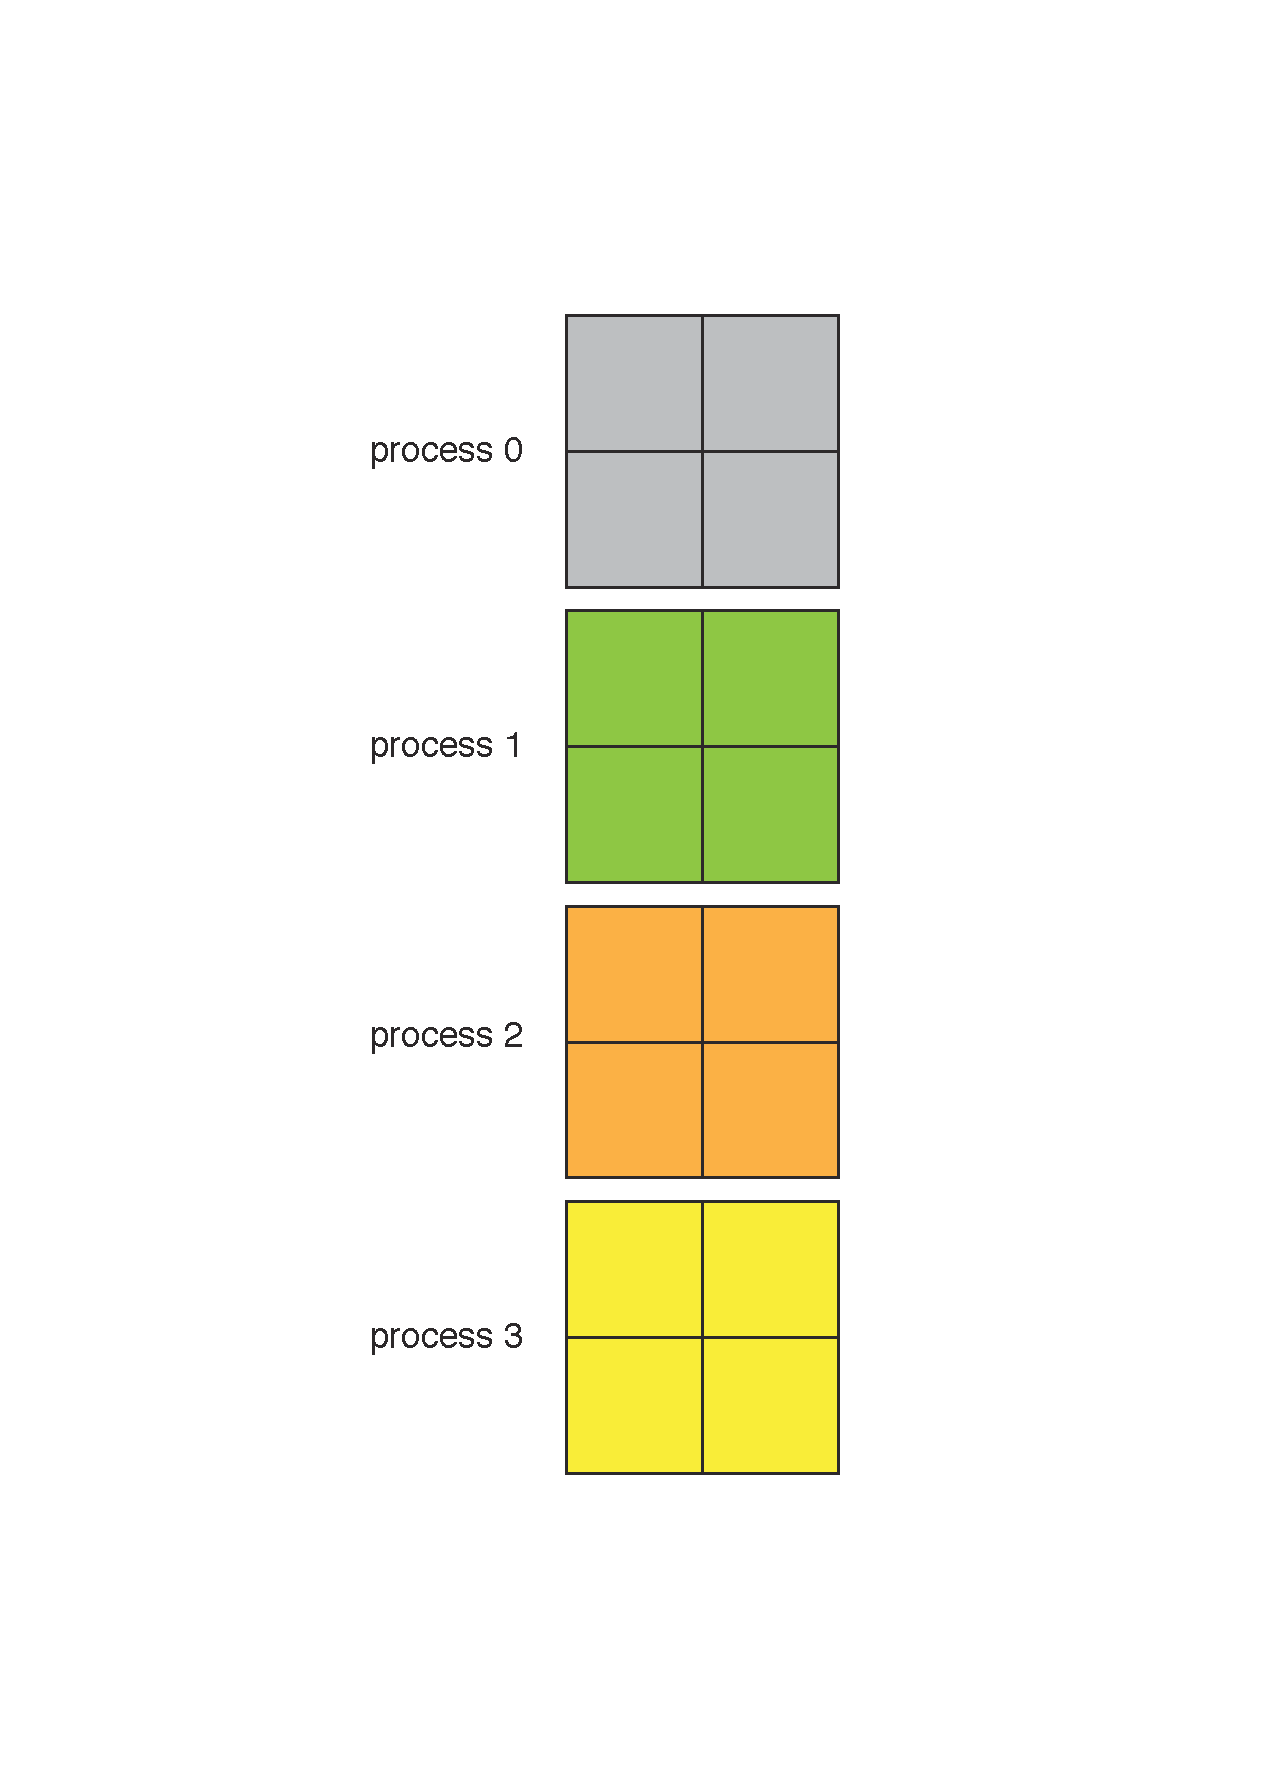
\includegraphics[height=0.45\textheight]{figure/local-view.pdf} \ \ \ \ \ \ \ \
    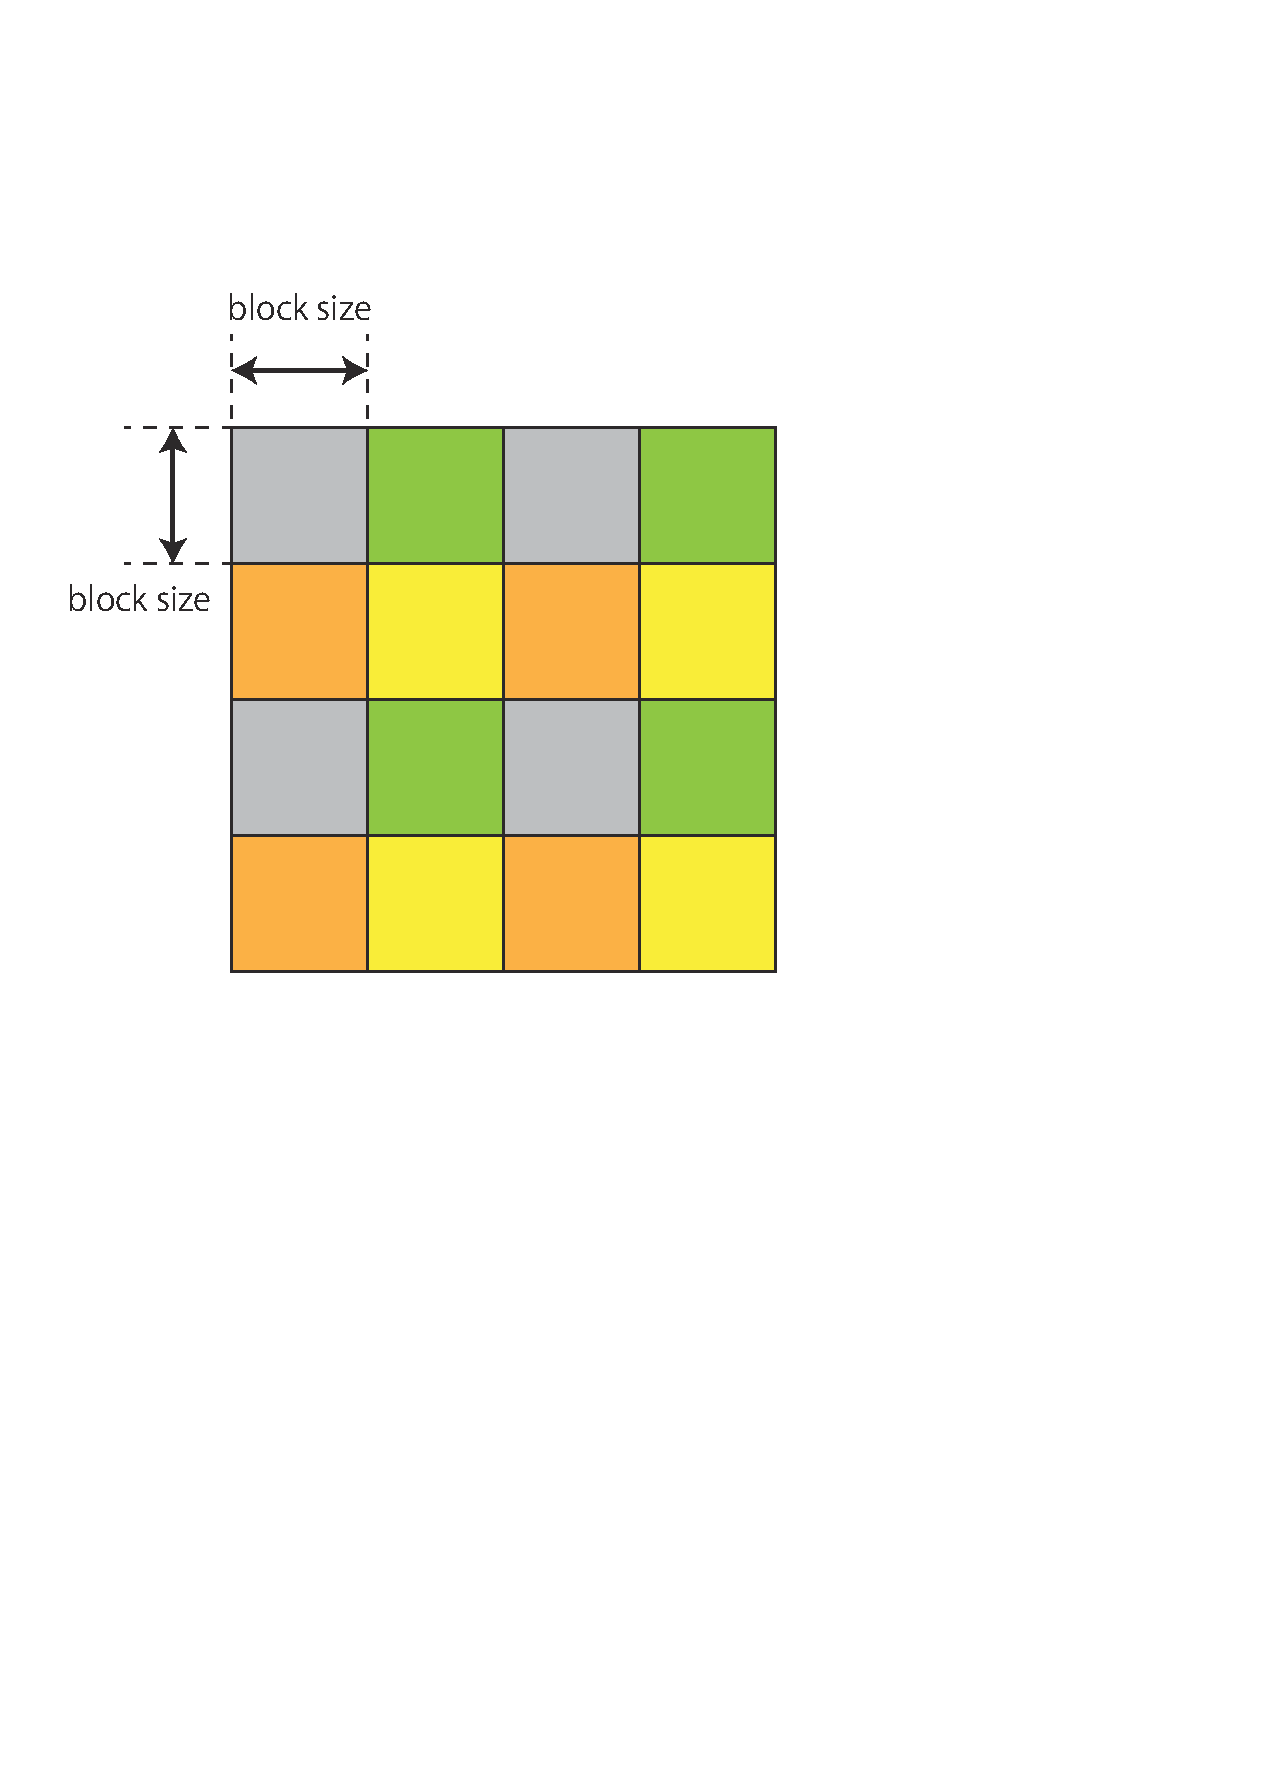
\includegraphics[height=0.35\textheight]{figure/global-view.pdf}
  \end{center}
  \item ScaLAPACKとELPAは任意のブロックサイズをサポート
  \item EigenExaとElementalは$1 \times 1$のみをサポート
  \end{itemize}
\end{frame}

\begin{frame}[c,fragile]
  \frametitle{rokko::grid クラス}
  \begin{itemize}
  \item \href{https://github.com/t-sakashita/rokko/blob/master/rokko/grid.hpp}{rokko/grid.hpp}
\begin{lstlisting}
namespace rokko {
extern struct grid_row_major_t {} grid_row_major;
extern struct grid_col_major_t {} grid_col_major;
class grid {
public:
  explicit grid(MPI_Comm comm_in = MPI_COMM_WORLD);
  template <typename GRID_MAJOR>
  grid(MPI_Comm comm_in, GRID_MAJOR const& grid_major);
  MPI_Comm get_comm() const { return comm; }
  int get_nprocs() const;
  int get_nprow() const;
  int get_npcol() const;
  int get_myrank() const;
  int get_myrow() const;
  int get_mycol() const;
  bool is_row_major() const;
  bool is_col_major() const;
  int calculate_grid_row(int proc_rank) const;
  int calculate_grid_col(int proc_rank) const;
};
}
\end{lstlisting}
  \end{itemize}
\end{frame}

\subsection{Rokkoインターフェースの仕様}

\begin{frame}[c,fragile]
  \frametitle{rokko::distributed\_matrix クラステンプレート}
  \begin{itemize}
  \item \href{https://github.com/t-sakashita/rokko/blob/master/rokko/distributed_matrix.hpp}{rokko/distributed\_matrix.hpp}
\begin{lstlisting}
namespace rokko {
template<typename MATRIX_MAJOR = rokko::matrix_row_major>
class distributed_matrix {
public:
  template<typename SOLVER>
  distributed_matrix(int m_global_in, int n_global_in, const grid& g_in, SOLVER const& solver_in);
  template<typename SOLVER>
  void initialize(int m_global_in, int n_global_in, const grid& g_in, SOLVER const& solver_in);
  int get_mb() const;
  int get_nb() const;
  int get_nprow() const;
  ...
  bool is_gindex_myrow(const int& global_i) const;
  bool is_gindex_mycol(const int& global_j) const;
  bool is_gindex(const int& global_i, const int& global_j) const;
  void set_local(int local_i, int local_j, double value);
  double get_local(int local_i, int local_j) const;
  void update_local(int local_i, int local_j, double value);
  void set_global(int global_i, int global_j, double value);
  double get_global(int global_i, int global_j) const;
};
}
\end{lstlisting}
  \end{itemize}
\end{frame}

\begin{frame}[c,fragile]
  \frametitle{distributed\_matrixの操作}
  \begin{itemize}
    %\setlength{\itemsep}{1em}
  \item 行列の掛け算 $C = \alpha A B + \beta C$
\begin{lstlisting}
  ...
  rokko::distributed_matrix<rokko::matrix_col_major> matA(dim, dim, g, solver);
  rokko::distributed_matrix<rokko::matrix_col_major> matB(dim, dim, g, solver);
  rokko::distributed_matrix<rokko::matrix_col_major> matC(dim, dim, g, solver);
  ...
  rokko::product(alpha, matA, transA, matB, transB, beta, matC);
\end{lstlisting}
  \item 分散行列の scatter と gather
\begin{lstlisting}
  rokko::localized_matrix<LOC_MAT_MAJOR> lmat(dim, dim);
  rokko::distributed_matrix<DIST_MAT_MAJOR> mat(dim, dim, g, solver);
  rokko::scatter(lmat, mat, root);
  rokko::gather(mat, lmat, root);
\end{lstlisting}
  \end{itemize}
\end{frame}

\begin{frame}[c,fragile]
  \frametitle{distributed\_matrixの生成}
  \begin{itemize}
    %\setlength{\itemsep}{1em}
  \item 要素毎に代入 (globalな添字)
\begin{lstlisting}
for(int global_i=0; global_i < mat.m_global; ++global_i) {
  for(int global_j=0; global_j < mat.n_global; ++global_j) {
    mat.set_global(global_i, global_j, f(global_i, global_j));
  }
}
\end{lstlisting}
  \item 要素毎に代入 (localな添字)
\begin{lstlisting}
for(int local_i = 0; local_i < mat.get_m_local(); ++local_i) {
  for(int local_j = 0; local_j < mat.get_n_local(); ++local_j) {
    int global_i = mat.translate_l2g_row(local_i);
    int global_j = mat.translate_l2g_col(local_j);
    mat.set_local(local_i, local_j, f(global_i, global_j));
  }
}
\end{lstlisting}
  \item 関数の値で行列を埋める
\begin{lstlisting}
mat.generate(f);
\end{lstlisting}
  \end{itemize}
\end{frame}

\begin{frame}[c,fragile]
  \frametitle{rokko::parallel\_dense\_solverクラス}
  \begin{itemize}
    %\setlength{\itemsep}{1em}
  \item 初期化
\begin{lstlisting}
rokko::parallel_dense_solver solver(name);
solver.initialize(argc, argv);
solver.finalize();
\end{lstlisting}
  \item 対角化 (行列は破壊される)
\begin{lstlisting}
rokko::distributed_matrix<matrix_col_major> mat(dim, dim, g, solver);
...
rokko::localized_vector evals(dim);
rokko::distributed_matrix<matrix_col_major> evecs(dim, dim, g, solver);
solver.diagonalize(mat, evals, evecs);
\end{lstlisting}
%  \item 登録されているソルバの一覧
%\begin{lstlisting}
%std::vector<std::string> names = rokko::parallel_dense_solver::solvers();
%\end{lstlisting}
  \end{itemize}
\end{frame}

\subsection{サンプルの実行}

\begin{frame}[c,fragile]
  \frametitle{対角化のサンプル}
  \begin{itemize}
    %\setlength{\itemsep}{1em}
%  \item MPI並列密行列ソルバーの一覧 \href{https://github.com/t-sakashita/rokko/blob/master/test/parallel_dense_solvers.cpp}{test/parallel\_dense\_solvers.cpp}
%\begin{lstlisting}[style=shstyle]
%./test/parallel_dense_solvers
%\end{lstlisting}
  \item C++ \href{https://github.com/t-sakashita/rokko/blob/master/sample/dense/frank_dense_mpi.cpp}{sample/dense/frank\_mpi.cpp}
\begin{lstlisting}[style=shstyle]
mpirun -np 4 ./sample/dense/frank_mpi eigen_exa_sx 5
\end{lstlisting}
  \item C \href{https://github.com/t-sakashita/rokko/blob/master/sample/dense/frank_dense_mpi.cpp}{sample/dense/frank\_mpi.cpp}
\begin{lstlisting}[style=shstyle]
mpirun -np 4 ./sample_c/dense/frank_mpi eigen_exa_sx 5
\end{lstlisting}
  \item Fortran \href{https://github.com/t-sakashita/rokko/blob/master/sample/dense/frank_dense_mpi.cpp}{sample/dense/frank\_mpi.cpp}
\begin{lstlisting}[style=shstyle]
mpirun -np 4 ./sample_fortran/dense/frank_mpi eigen_exa_sx 5
\end{lstlisting}

  \end{itemize}
\end{frame}

\section{疎行列向け並列ソルバ}

\subsection{基本概念}

\begin{frame}[c,fragile]
  \frametitle{CRS(Compressed Row Storage)方式}
%疎行列の非ゼロ成分のみを求め固有値ソルバに渡す方法である.
%この方法で用いられる疎行列の代表的な格納方式には,CRS方式(Compressed Row Storage, 圧縮行格納方式)がある.
各行ごとに非ゼロ成分とその列添字を格納する方法

\begin{rei}%
\begin{align*}
\begin{bmatrix}
7.1 & 5.2 & 0 & 0 \\
0 & 0 & 0 & 6.4 \\
0.2 & 0 & 0 & 4.3 \\
0 & 0 & 0.5 & 0
\end{bmatrix}
\end{align*}
CRS方式による表現:
\begin{itemize}
%\item 非ゼロ成分に対する行添字$= [1, 1, 2, 3, 3, 4] $
\item 各行ごとの非ゼロ成分の個数 $num\_nonzero\_cols = [2, 1, 2, 1]$
\item 非ゼロ成分に対する列添字 $nonzero\_cols = [1, 2, 4, 1, 4, 3]$
%\begin{bmatrix}
%1 & 2 \\
%4 \\
%1 & 4 \\
%3
%\end{bmatrix}$
\item 非ゼロ行列成分 $values = [7.1, 5.2, 6.4, 0.2, 4.3, 0.5]$
\end{itemize}
\end{rei}

MPI並列化は行単位

\end{frame}

\subsection{Rokkoインターフェースの仕様}

\begin{frame}[c,fragile]
  \frametitle{rokko::distributed\_crs\_matrix クラステンプレート}
\begin{lstlisting}
namespace rokko {
class distributed_crs_matrix {
public:
  void insert(int row, std::vector<int> const& cols, std::vector<double> const& values);
  void insert(int row, int col_size, int* cols, double* const values);
  void complete();
  int get_dim() const;
  int num_local_rows() const;
  int start_row() const;
  int end_row() const;
  void print() const;
};
}
\end{lstlisting}
\end{frame}


\begin{frame}[c,fragile]
  \frametitle{rokko::distributed\_crs\_matrix クラス(使用例)}
\begin{lstlisting}
  rokko::parallel_sparse_solver solver("anasazi");
  int dim = 4;
  rokko::distributed_crs_matrix mat(dim, dim, solver);

  int num_nonzero_cols[] = {2, 1, 2, 1};
  int nonzero_cols[] = {0, 1, 3, 0, 3, 2};
  double values[] = {7.1, 5.2, 6.4, 0.2, 4.3, 0.5};

  int current = 0;
  for (int row = 0; row < dim; ++row) {
    mat.insert(row, num_nonzero_cols[row], &nonzero_cols[current], &values[current]);
    current += num_nonzero_cols[row]; 
  }
  mat.complete();
  mat.print();
\end{lstlisting}
\noindent
サンプルの実行
  \begin{itemize}
  \item Anasaziの場合
\begin{lstlisting}[style=shstyle]
mpirun -np 4 ./sample/sparse/distributed_crs_matrix anasazi
\end{lstlisting}
  \item SLEPcの場合
\begin{lstlisting}[style=shstyle]
mpirun -np 4 ./sample/sparse/distributed_crs_matrix slepc
\end{lstlisting}
  \end{itemize}
\end{frame}


\begin{frame}[c,fragile]
  \frametitle{Matrix free方式}
たいていの疎行列向け固有値ソルバでは、固有値分解を行うべき行列とベクト
ル積を行うルーチンのみが必要である。
行列をあらわに作る必要がない。
 \\
 \\
\noindent
rokko::distributed\_mfreeを継承し、
  \begin{itemize}
   \item multiply(const double* x, double* y)関数
   \item void diagonal(double* x)関数 (SLEPcの場合) 
  \end{itemize}
を持つクラスを定義する。
\end{frame}

\begin{frame}[c,fragile]
  \frametitle{Matrix free方式(例)}
\begin{lstlisting}
class heisenberg_op : public rokko::distributed_mfree {
public:
  heisenberg_op(int L, const std::vector<std::pair<int, int> >& lattice) : L_(L), lattice_(lattice) {
    comm_ = MPI_COMM_WORLD;
    int nproc;
    MPI_Comm_size(comm_, &nproc);
    int n = nproc;
    int p = -1;
    do {
      n /= 2;
      ++p;
    } while (n > 0);
    local_N = 1 << (L-p);
    buffer_.assign(local_N, 0);
    dim_ = 1 << L;
  }
  ~heisenberg_op() {}

  void multiply(const double* x, double* y) const {
    rokko::heisenberg_hamiltonian::multiply(comm_, L_, lattice_, x, y, &(buffer_[0]));
  }
  int get_dim() const {
    return dim_;
  }
  int get_num_local_rows() const {
    return local_N;
  }
\end{lstlisting}
\end{frame}

\begin{frame}[c,fragile]
  \frametitle{Matrix free方式(例の続き)}
\begin{lstlisting}
private:
  MPI_Comm comm_;
  mutable std::vector<double> buffer_;
  int L_;
  int local_N;
  std::vector<std::pair<int, int> > lattice_;
  int dim_;
};
\end{lstlisting}
\end{frame}


\begin{frame}[c,fragile]
  \frametitle{rokko::parallel\_sparse\_solverクラス(疎行列、MPI並列版)}
  \begin{itemize}
    %\setlength{\itemsep}{1em}
  \item 初期化
\begin{lstlisting}
rokko::parallel_sparse_solver solver(name);
solver.initialize(argc, argv);
solver.finalize();
\end{lstlisting}
  \item 対角化(CRS行列の場合)
\begin{lstlisting}
rokko::distributed_crs_matrix mat(dim, dim, solver);
...
solver.diagonalize(mat, num_evals, block_size, max_iters, tol);
\end{lstlisting}
  \item 対角化(Matrix Freeの場合)
\begin{lstlisting}
heisenberg_op  mat(L, lattice);
solver.diagonalize(mat, num_evals, block_size, max_iters, tol);
\end{lstlisting}

  \item 固有値・固有ベクトルの取り出し
\begin{lstlisting}
int i;
solver.eigenvalue(i);
std::vector<double> eigvec;
solver.eigenvector(i, eigvec);
\end{lstlisting}
%  \item 登録されているソルバの一覧
%\begin{lstlisting}
%std::vector<std::string> names = rokko::parallel_sparse_solver::solvers();
%\end{lstlisting}
  \end{itemize}
\end{frame}



\section{量子スピン系の対角化}

\begin{frame}[c,fragile]
  \frametitle{量子スピン系の対角化(密行列、逐次・MPI版)}
  \begin{itemize}
    %\setlength{\itemsep}{1em}
  \item Heisenberg模型(逐次版) \href{https://github.com/t-sakashita/rokko/blob/master/sample/dense/heisenberg_mpi.cpp}{sample/dense/heisenberg.cpp}
\begin{lstlisting}[style=shstyle]
./sample/dense/heisenberg lapack
\end{lstlisting}
  \item Heisenberg模型(MPI版) \href{https://github.com/t-sakashita/rokko/blob/master/sample/dense/heisenberg_mpi.cpp}{sample/dense/heisenberg\_mpi.cpp}
\begin{lstlisting}[style=shstyle]
mpirun -np 4 ./sample/dense/heisenberg_mpi eigen_exa_sx
\end{lstlisting}
  \item XYZ模型(逐次版) \href{https://github.com/t-sakashita/rokko/blob/develop/sample/dense/xyz_dense.cpp}{sample/dense/xyz.cpp}
\begin{lstlisting}[style=shstyle]
./sample/dense/xyz_dense lapack $HOME/rokko-0.1/test/input_data/xyz_1hexagon.ip
\end{lstlisting}
  \item XYZ模型(MPI) \href{https://github.com/t-sakashita/rokko/blob/develop/sample/dense/xyz_mpi.cpp}{sample/dense/xyz\_mpi.cpp}
\begin{lstlisting}
mpirun -np 4 ./sample/dense/xyz_mpi eigen_exa_sx $HOME/rokko-0.1/test/input_data/xyz_1hexagon.ip
\end{lstlisting}
  \end{itemize}
\end{frame}

\begin{frame}[c,fragile]
  \frametitle{量子スピン系の対角化(疎行列、MPI版)}
  \begin{itemize}
    %\setlength{\itemsep}{1em}
  \item Heisenberg模型(CRS) \href{https://github.com/t-sakashita/rokko/blob/master/sample_anasazi/heisenberg_crs_mpi.cpp}{sample/sparse/heisenberg\_crs\_mpi.cpp}
\begin{lstlisting}[style=shstyle]
mpirun -np 4 ./sample/sparse/heisenberg_crs_mpi
\end{lstlisting}
  \item Heisenberg模型(MatFree) \href{https://github.com/t-sakashita/rokko/blob/master/sample_anasazi/heisenberg_mfree_mpi.cpp}{sample/sparse/heisenberg\_mfree\_mpi.cpp}
\begin{lstlisting}[style=shstyle]
mpirun -np 4 ./sample/sparse/heisenberg_mfree_mpi
\end{lstlisting}
  \item XYZ模型(CRS) \href{https://github.com/t-sakashita/rokko/blob/master/sample/sparse/xyz_crs_mpi.cpp}{sample/sparse/xyz\_crs\_mpi.cpp}
\begin{lstlisting}[style=shstyle]
mpirun -np 4 ./sample/sparse/xyz_crs_mpi
\end{lstlisting}
  \item XYZ模型(Matfree) \href{https://github.com/t-sakashita/rokko/blob/master/sample/sparses/xyz_mfree_mpi.cpp}{sample/sparse/xyz\_mfree\_mpi.cpp}
\begin{lstlisting}[style=shstyle]
mpirun -np 4 ./sample/sparse/xyz_mfree_mpi
\end{lstlisting}
  \end{itemize}
\end{frame}

\section{TITPACK2へのRokko組み込み実習}

\begin{frame}[c,fragile]
  \frametitle{TITPACKの概要}
\end{frame}

\begin{frame}[c,fragile]
  \frametitle{ディレクトリ構成}

\dirtree{%
 .1 \href{https://github.com/t-sakashita/rokko/tree/develop/tutorial/}{tutorial}.
 .2
 \href{https://github.com/t-sakashita/rokko/tree/develop/tutorial/titpack}{titpack}.
 .3
 \href{https://github.com/t-sakashita/rokko/tree/develop/tutorial/titpack/00_original}{00\_original}
 $\cdots$ 独自固有値ソルバのFortran版.
 .3
 \href{https://github.com/t-sakashita/rokko/tree/develop/tutorial/titpack/01_lapack}{01\_lapack}
 $\cdots$ FortranのままLAPACK化.
 .3
 \href{https://github.com/t-sakashita/rokko/tree/develop/tutorial/titpack/01_lapack_cxx}{01\_lapack\_cxx}
 $\cdots$ C++でLAPACK版.
 .3
 \href{https://github.com/t-sakashita/rokko/tree/develop/tutorial/titpack/02_refactored_cxx}{02\_refactored\_cxx}
 $\cdots$ C++晩のリファクタリング版.
 .3
 \href{https://github.com/t-sakashita/rokko/tree/develop/tutorial/titpack/03_rokko_cxx}{03\_rokko\_cxx}
 $\cdots$ C++でRokko化.
}
\end{frame}


\section{アプリケーションからのRokkoの利用}

\begin{frame}[c,fragile]
  \frametitle{CMakeによるRokkoライブラリの取り込み方法}
\end{frame}

\begin{frame}[c,fragile]
  \frametitle{MakefileによるRokkoライブラリの取り込み方法}
\end{frame}


\end{document}




%\section{ALPS/Baristaパッケージ}
%\section{MateriAppsとMateriApps LIVE!}

\begin{frame}
  \frametitle{テスト}
  \begin{itemize}
    %\setlength{\itemsep}{1em}
  \item テスト
  \end{itemize}
\end{frame}

